\hypertarget{chapter-7---bwt}{%
\section{Chapter 7 - BWT}\label{chapter-7---bwt}}
\label{sec:bwt}
When working with large text corpora, one usually faces the problem of the scarcity of storage space as well as the need for quickly searching for relevant information. For a long time these two requirements have been perceived as conflicting in the sense that one cannot use text compression and still support efficient search queries and conversely, an indexed text cannot be significantly smaller than the plain one. To the surprise of many, both of these demands can be met simultaneously with the so-called \bwt{} \cite{burrows1994block}. In the following text, we will first define the \bwt{} and outline some of its properties, then in subsections \ref{subseq:bwt_compression} and \ref{subseq:bwt_backward_search} we will describe how it facilitates compression and how it can be used for text indexing, respectively. Subsection \ref{subseq:bwt_apps} briefly lists a selection of impactful applications built around the mentioned ideas.

The \bwt{} (BWT) of a null-terminated string $T$ of length $n$ is a permutation of $T$ formed by the characters that precede the suffixes of $T$ sorted in the \lex{} order, while we treat $T$ as circular. It was originally introduced by Burrows and Wheeler in 1994 \cite{burrows1994block} for the purpose of text compression. Formally, let us denote $M$ to be the matrix the rows of which consist of all \lex{ally} sorted rotations of $T$, or more specifically, $M = \big( m_{i,j} \big)_{1 \leq i, j \leq n}$, where $m_{i,1} \ldots m_{i, n} = T[SA[i]..n]T[1..SA[i]-1]$. Moreover, let $F = m_{1,1} \ldots m_{n, 1}$ resp.~$L = m_{1,n} \ldots m_{n, n}$ be the string consisting of first resp. last column of $M$. Then we call $L$ the BWT of $T$ and denote it $BWT(T)$. Using as example the text $T = \texttt{TATGTTTTCGATG\$}$, we have $BWT(T) = L = \texttt{GGTTTCT\$TAATTG}$ and $F = \texttt{\$AACGGGTTTTTTT}$. 
As one can observe, $F$ can be obtained by simply sorting the characters of $T$. Fig. \ref{fig:bwt} depicts the complete matrix $M$.

\begin{figure}[!ht]
\centering
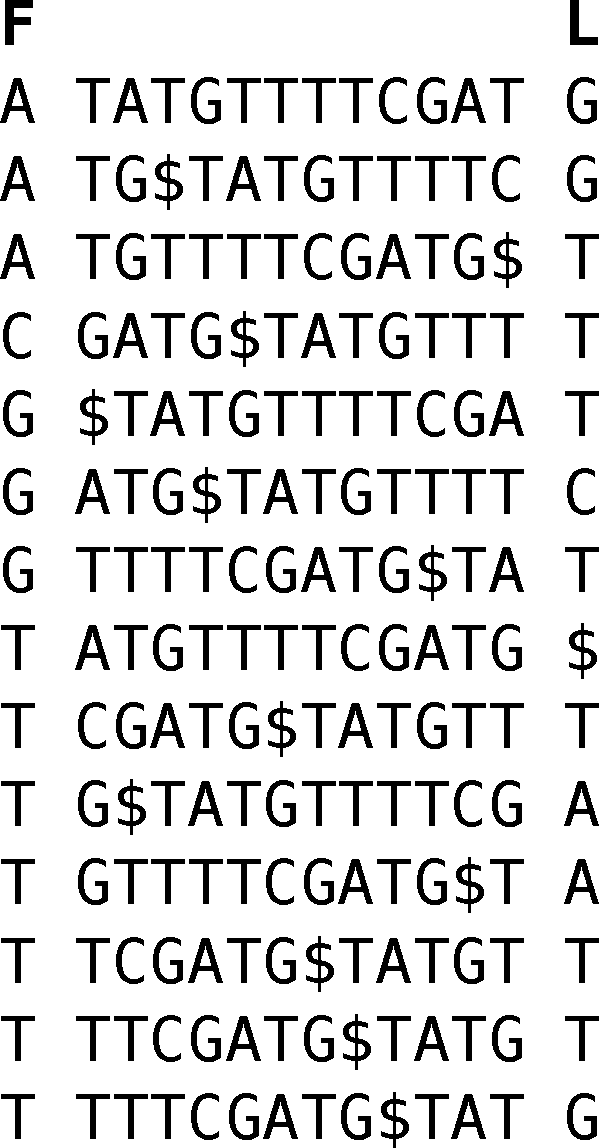
\includegraphics[width=0.2\textwidth]{images/bwt.pdf}
\label{fig:bwt}
\caption[A BWT matrix example.]{An example of a matrix $M$ from the BWT example  in Section \ref{sec:bwt}. Inspired by Bentley et al. \cite{bentley2019complexity}.}
\end{figure}


Interestingly enough, the BWT is also invertible, i.e. we can reconstruct $T$ from just $BWT(T)$. The reconstruction is done by means of the following observations. Firstly, it holds that the $k$-th occurrence of a character $c$ in $L$ corresponds to the $k$-th occurrence the same character in $F$. This is true because from the inequality $cx \prec cy$ it must hold that $x \prec y$ and so trivially also $xc \prec yc$. Therefore, for any given suffix $T[i\ldots n]$ corresponding to the position $j$ in $L$ resp. $M$ (i.e. $SA^{-1}[i+1] = j$) and $L[j]$ is the $k$-th occurrence of the character in $L[1 \ldots j]$, we can find the position in $L$ corresponding to the suffix $T[i-1 \ldots n]$ by locating the $k$-th occurrence of $L[j]$ in $F$. Since the $k$-th row of $M$ that ends on $L[j]$ is essentially $T[i \ldots n]$ cyclically shifted rightwards for one character, we now know the corresponding position in $L$ for $T[i-1 \ldots n]$. These observations can be summarized in a bijective mapping between the columns $L$ and $F$, hence it is known by the name $LF$-mapping and defined as


\begin{equation}
    \text{LF}(i) =  \sum_{1 \leq j \leq n} [L[j] \prec L[i]] + \sum_{1 \leq j \leq i} [L[i] = L[j]],
\end{equation}

\hypertarget{construction-by-induced-sorting}{%
\subsection{Construction by Induced Sorting}\label{construction-by-induced-sorting}}

We can construct the BWT from SA by $BWT[i] = SA[(i-1) \text{ mod } n]$, but that requires storing the $SA$. However, SACAs are not very space-efficient and require at least $n \log n + n \log \sigma$ bits of memory (SA + $S$), which is not feasible for large memories. For this reason this is why it is more advantageous to use direct BWT construction algorithms, especially for large files/alphabets. In fact, IS can be adapted to compute the BWT directly instead of the SA.

\subsection{Compression}
\label{subseq:bwt_compression}
In practice, large texts are often redundant and so the occurrences of a substring are oftentimes being preceded by only a few distinct characters. If we, for example, take the string \textit{ssion}, there is only a few characters ($e$, $i$, etc.) that could precede it to form a valid English word. Combining this with the fact that the characters in $L$ precede lexicographically sorted -- and therefore similar -- suffixes, we observe intervals in which only a few characters occur. This dramatically decreases the higher-order entropy of $L$ and leads to the creation of long runs -- maximal unary substrings. The presence of long runs enables the BWT to be much more compressible in practice, since any run $a\ldots a$ of length $x$ can be simply encoded as $xa$, which is also the basis of the \textit{run-length encoding (RLE)}. We note that RLE is usually only the second stage of encoding done to a BWT and is often preceeded by a move-to-front transformation (MTF) \cite{ryabko1980data, bentley1986locally} as the first stage and succeeded by an efficient prefix-free code, such as Huffman code \cite{burrows1994block} as the third stage. The described procedure is essentially the basis of the popular \texttt{bzip2} \cite{seward1996bzip2} compression algorithm.

\subsection{Backward Search}
\label{subseq:bwt_backward_search}
Although BWT was originally developed for the purpose of data compression, it was extended into a fully functional text index data structure in 2000 by Ferragina and Manzini \cite{fmindex2000manzini} under the the name of FM-index. FM-index of a string $T$ consists of a compressed representation of $BWT(T)$ enriched with several auxiliary data structures that enable efficient search queries within the compressed space.

In more detail, the need for the auxiliary data stems from the goal of supporting quick enough computation of the $LF$ mapping. Considering that the alphabet size $\sigma$ is small with respect to $n$, e.g. constant-sized as was assumed by Ferragina and Manzini \cite{fmindex2000manzini}, the $C$ array of cumulative character frequencies is also small and hence can be stored as is. The efficiency of the $LF$ mapping is therefore determined by the way we support the $\texttt{rank}$ query. Ferragina and Manzini proposed a $O(1)$ time solution of this problem using $O((n/(\log n)) \log \log n)$ bits of additional space in terms of a RAM model with the word size of $w = \Theta(\log n)$ \cite{fmindex2000manzini}, but also other efficient solutions are known.

Ferragina and Manzini describe a \textit{backward search} procedure, which allows to efficiently search for a pattern within the FM-index. We will now summarize the method with regards to the two types of queries supported: \textit{count} and \textit{locate}.

\subsubsection{Count Queries}
As before, let $P = P[1] \ldots P[m]$ be the pattern of which we want to count the number of occurrences in text $T$. We will use the observation that the entries of the matrix $M$ containing a suffix $P[i \ldots m]$ as a prefix correspond to: $a)$ exactly the occurrences of $P[i \ldots m]$ in $T$; $b)$ an interval $[s,e] \subseteq [1, n]$. We will therefore maintain the invariant that for each $i$ we have the interval $[s_i, e_i]$, where $s_i$ resp. $e_i$ points to the lexicographically first resp. last row prefixed by $P[i \ldots m]$. We start with $[s_{m+1}, e_{m+1}] = [1, n]$ representing the occurrences of prefix $P[m+1 \ldots m] = \varepsilon$, and for each  $i = m, \ldots, 1$, we obtain the interval $[s_i, e_i]$ of suffixes of $T$ which contain $P[i \ldots m]$ as a prefix as $[C[P[i]] + \texttt{rank}(L, P[i],s_{i+1}), C[P[i]] + \texttt{rank}(L, P[i], e_{i+1})]$. Upon finishing the iterations, we end up with the interval $[s_1, e_1]$ of suffixes of $T$ which contain $P$ as a prefix, i.e. precisely the occurrences of $P$ in $T$. The count query takes only $O(m)$ time and requires $|L| + O((n/(\log n)) \log \log n)$ of bits of space \cite{fmindex2000manzini}.

\subsubsection{Locate Queries}
In order to find the locations of the occurrences of $P$ in $T$, we can first find the interval $[s_1, e_1]$ by the backwards search as in the counting query. However, this interval does not inherently contain the information about the actual positions of the occurrences of $P$. A valid option would be to use the interval $[s_1, e_1]$ to query the suffix array of $T$, however, storing the SA would require additional space of $O(n \log n)$. Ferragina and Manzini \cite{fmindex2000manzini} proposed storing the $SA$ samples at regular intervals of $T$ of length $k \geq 0$ such that $k = \Theta(\log n)$. To locate an occurrence of $P$ corresponding to $SA[i]$, the $LF$ mapping is used to find the nearest stored $SA[j]$ entry to which the offset (the number of $LF$ used mappings) is added. Using suitable data structure to store the $SA$ samples, all the $occ$ occurrences of $P$ in $T$ can be listed in $O(m + occ \log^2 m)$ using $5 H_k(T) + O(\frac{\log \log n}{\log})$ space. This approach was refined in the same article to running time of $O(m + \log^{\varepsilon} n)$ and $O(H_k(T) + \frac{\log \log n}{\log^{\varepsilon} n})$ space for a constant $\varepsilon > 0$.

\subsection{Wavelet Trees}

\subsection{Matching Statistics}
The calculation of MS for strings $S^1, S^2$ using a BWT is quite simple.
We assume that we have already computed the BWT of $S^1$ as well as the LCP array and preprocessed it so that we can compute the parent interval of any particular lcp interval in $O(1)$ time.
Then it suffices to match $S^2$ in a \textit{backwards fashion} against the BWT of $S^1$ while keeping the length of match and computing the parent interval whenever we encounter an empty interval.
The pseudocode is given in Alg. \ref{alg:BWTMS}.

\begin{figure}[!ht]
    \centering
    \begin{minted}{python}
    n1, n2 = len(S1), len(S2)
    MS = [-1]*n2
    lb, rb = 0, n1-1
    p2 = n2-1
    
    while p2 >= 0:
        lb, rb = backwardstep(lb, rb, S2[p2])
        if lb == n1+1 and l > 0: # we have an empty interval
            lb, rb = parent(lb, rb)
            l = LCP[rb]
        else:
            l += 1
            MS[p2] = l
            p2 -= 1
    \end{minted}
    \caption{Matching statistics calculation using the BWT.}
    \label{alg:BWTMS}
\end{figure}

Let us now analyze the time complexity of Alg. \ref{alg:BWTMS}.
In each iteration of the \texttt{while} loop, we either decrement \texttt{p2} and increment the current $\lcp$ value $\ell$ or decrease $\ell$ by at least $1$.
The total amount of times $\ell$ is decreased is bounded by the number of the total increase of $\ell$, which in turn is bounded by $n_2$.
Hence if we assume the BWT of $S_1$, the LCP array of $S_1$ and other auxiliary structures are already computed, the total running time of Alg. \ref{alg:BWTMS} is $O(n_2)$.

\subsection{MEMs}
In many applications we are only interested in MEMs between strings $S^1, S^2$ greater than a certain length $L$.
Here we show how to compute these using the BWT.
The approach is very similar to that of computing MSs using the BWT.
We also match $S^2$ in the backwards fashion against the BWT of $S^1$.
We will, however, keep track of the current \textit{matching path}, which is a list of intervals in which every entry $\ell - [i,j]$ satisfies $\ell > L$.

After we encounter an empty interval, we start scanning through the matching path and output MEMs.
In more detail, we know that that for each interval $\ell - [i,j]$ in the matching path, the indices $k \in [i, j]$ for which $\bwt[k] \neq S^2[p_2 - 1]$ are the MEMs longer than $L$.
We subsequently move on to the parent $lb, rb$ interval of $[i, j]$ and if its LCP values is greater than $L$, we output those indices $k \in [i, j]$ for which $\bwt[k] \neq S^2[p_2 - 1]$ and simultaneously $k \notin [i, j]$.
Then we proceed with accordingly.
The procedure is sketched in Alg. \ref{alg:BWTMEMs}.

\begin{figure}[!ht]
    \centering
    \begin{minted}{python}
    n1, n2 = len(S1), len(S2)
    MS = [-1]*n2
    lb, rb = 0, n1-1
    p2 = n1-1
    path = []
    MEMs = [] # the output
    
    while p2 >= 0:
        lb, rb = backwardstep(lb, rb, S2[p2])
        if lb == n1+1: # we have an empty interval
            lb, rb, l = parent(lb, rb)
            # output all MEMs of length > L
            for i, j in path:
                while l > L:
                    bad_l, bad_r = j+1, i 
                    for k in [i, j] - [bad_l, bad_r]:
                        if BWT[k] != S2[p2]:
                            MEMs.append( (k, p2, l) )
                        i, j, l = parent(i, j)
            path = []
        else:
            l += 1
            if l > L:
                path.append( (i, j, l) )
            MS[p2] = l
            p2 -= 1
    \end{minted}
    \caption{Calculation of all MEMs of length $> L$ using the BWT.}
    \label{alg:BWTMEMs}
\end{figure}

\subsection{Shortest Unique Substrings}
\label{sec:SUSBWT}
We can calculate SUSs using a BWT by modifying the algorithm to compute the LCP values.
When we fill in a $\lcp[rb]$ entry, we check whether $rb-1$ was already set and compare these two values.
Similarly for the value $rb+1$, if it was already set, we can compare the current value with $\lcp[rb+1]$ and output the SUS.
We also need to keep track of the position of the suffix $S_{\ell}$, since that one is always unique and hence not interesting.
We do that by keeping the index of the $S_{\ell}$ in the BWT, which is $0$ for $\ell = 0$ and when we move to $\ell : \ell + 1$, we update it by $idx = \text{LF}(idx)$.
The complete algorithm is as follows:

\begin{minted}{python}
LCP = [-2]*(n+1) # -2 stands for yet unassigned value
for c in C:
    Q.push( (C[c]+1, C[c+1]) )
size = len(C)
l = 0
idx = 0
while not Q.empty():
    lb, rb = Q.pop()
    if LCP[rb] == -2:
        LCP[rb] = l
        if LCP[rb-1] != -2 and SA[rb-1] != idx:
            m = max(LCP[rb-1], LCP[rb]) + 1
            output(SA[rb-1], m)
        if LCP[rb+1] != -2 SA[rb-1] != idx:
            m = max(LCP[rb], LCP[rb]+1) + 1
            output(SA[rb], m)
        for (i, j) in get_intervals(BWT, lb, rb):
            Q.push(i, j)
    idx += 1
    size -= 1
    idx = LF(idx)
    if size == 0:
        size = Q.size()
        l += 1
\end{minted}

In fact, if we are not interested in the LCP values at all, we may simply use a bitvector $B$, in which $B[i] = 1$ if and only if $\lcp[i] \neq -2$.
We can do this, since we are filling the $\lcp$ array in increasing order from $\ell = 0$ and when we fill the $\lcp[i]$ entry, we know that other filled entries have the same or less value.
The time complexity remains the same as in the $\lcp$ values computation as we do only constant time overhead in each iteration in the while cycle.